\chapter{Cài đặt và tích hợp hệ thống}

Chương này trình bày cách hiện thực thiết kế ở Chương 2, từ tổ chức mã nguồn, cài đặt ba thành phần chính đến tích hợp các luồng chức năng xuyên suốt hệ thống.

\medskip

\section{Tổ chức mã nguồn và môi trường triển khai}

Dự án được tổ chức dưới dạng kho mã nguồn hợp nhất, sử dụng pnpm workspace và Turborepo để quản lý các ứng dụng cùng gói mã dùng chung \cite{pnpm,turborepo}. Cấu trúc này giúp một thay đổi liên quan tới nhiều thành phần, chẳng hạn VTON, có thể được theo dõi thống nhất mà vẫn duy trì ranh giới trách nhiệm rõ ràng.

\medskip

\begin{table}[H]
\centering
\caption{Vai trò các thư mục chính trong mã nguồn dự án}
\label{tab:source-directories}
\begin{tabularx}{\textwidth}{L{3.8cm}Y}
\toprule
\textbf{Thư mục} & \textbf{Vai trò} \\
\midrule
\code{apps/web} & Ứng dụng Next.js gồm cửa hàng, AI Stylist, tủ đồ, hồ sơ AI và giao diện thử đồ. \\
\addlinespace
\code{apps/api-medusa} & Hệ thống nghiệp vụ MedusaJS, gồm API tùy chỉnh, quy trình nghiệp vụ, mô-đun cá nhân hóa, bộ chuyển đổi RabbitMQ và bộ quản lý SSE. \\
\addlinespace
\code{apps/ai-service} & Dịch vụ FastAPI thực hiện tìm kiếm LanceDB, gọi Gemini, sinh vector nhúng và xử lý VTON. \\
\addlinespace
\code{packages/shared-types} & Chứa các lược đồ Zod dùng chung cho thông điệp xử lý ảnh và phản hồi lỗi. \\
\addlinespace
\code{docker} & Cấu hình Docker Compose cho PostgreSQL, Redis và RabbitMQ. \\
\bottomrule
\end{tabularx}
\end{table}

\begin{figure}[H]
\centering
\resizebox{0.96\textwidth}{!}{%
\begin{tikzpicture}
    \node[diagram user, minimum width=3.0cm] (browser) at (0,0) {Trình duyệt};

    \node[diagram service, minimum width=3.3cm] (web) at (4.2,0) {Next.js\\\code{localhost:3000}};
    \node[diagram service, minimum width=3.3cm] (medusa) at (8.8,0) {MedusaJS\\\code{localhost:9000}};
    \node[diagram ai, minimum width=3.3cm] (fastapi) at (13.4,0) {FastAPI\\\code{localhost:8000}};

    \node[diagram data, minimum width=3.0cm] (postgres) at (4.8,-3.4) {PostgreSQL 15\\cổng 5432};
    \node[diagram data, minimum width=2.8cm] (redis) at (8.5,-3.4) {Redis\\cổng 6379};
    \node[diagram queue, minimum width=3.1cm] (rabbit) at (12.2,-3.4) {RabbitMQ\\5672 / 15672};
    \node[diagram data, minimum width=3.1cm] (lance) at (16.1,-3.4) {LanceDB\\vector cục bộ};
    \node[diagram data, minimum width=3.1cm] (files) at (20.0,-3.4) {Tệp tĩnh\\kết quả VTON};

    \node[diagram ai, minimum width=3.0cm] (gemini) at (11.0,3.5) {Gemini API};
    \node[diagram ai, minimum width=3.2cm] (replicate) at (16.0,3.5) {Replicate\\FLUX.2 Pro};

    \begin{scope}[on background layer]
        \node[diagram group, fill=gray!2, fit=(web)(medusa)(fastapi)(postgres)(redis)(rabbit)(lance)(files),
              label={[font=\small\bfseries]above left:Môi trường phát triển cục bộ}] {};
        \node[diagram group, fill=violet!2, fit=(gemini)(replicate),
              label={[font=\small\bfseries]above:Dịch vụ đám mây}] {};
    \end{scope}

    \draw[diagram arrow, <->] (browser) -- (web);
    \draw[diagram arrow, <->] (web) -- (medusa);
    \draw[diagram arrow, <->] (medusa) -- (fastapi);
    \draw[diagram arrow, <->] (medusa) -- (postgres);
    \draw[diagram arrow, <->] (medusa) -- (redis);
    \draw[diagram async, <->] (medusa) -- (rabbit);
    \draw[diagram async, <->] (rabbit) -- (fastapi);
    \draw[diagram arrow, <->] (fastapi) -- (lance);
    \draw[diagram arrow, <->] (fastapi) -- (files);
    \draw[diagram arrow, <->] (fastapi) -- (gemini);
    \draw[diagram arrow, <->] (fastapi) -- (replicate);
\end{tikzpicture}%
}
\caption{Sơ đồ triển khai hệ thống trong môi trường phát triển cục bộ}
\label{fig:local-deployment}
\end{figure}


\medskip

Trong cấu trúc này, ứng dụng web tiếp nhận thao tác của người dùng, Medusa điều phối nghiệp vụ và dịch vụ AI xử lý ngôn ngữ, truy hồi vector cùng sinh ảnh.

\section{Cài đặt giao diện Next.js}

Giao diện được xây dựng bằng Next.js 14 App Router, React 18, Tailwind CSS và Zustand \cite{nextjs,react,tailwind,zustand}. Các trang được tổ chức theo hành trình sử dụng: duyệt sản phẩm, thiết lập hồ sơ AI, quản lý tủ đồ, nhận tư vấn phối đồ, thử đồ và chuyển sang thanh toán mô phỏng.

\medskip

Trạng thái phía giao diện được chia theo miền nghiệp vụ. \code{useCartStore} quản lý giỏ hàng; \code{useStylistStore} quản lý hội thoại và phương án phối đồ; \code{useVTONStore} quản lý ảnh người dùng, bộ xử lý được chọn, trạng thái tác vụ và ảnh kết quả. Cách phân chia này giới hạn phạm vi cập nhật giao diện và giúp mỗi kho trạng thái có trách nhiệm rõ ràng.

\medskip

\begin{figure}[H]
    \centering
    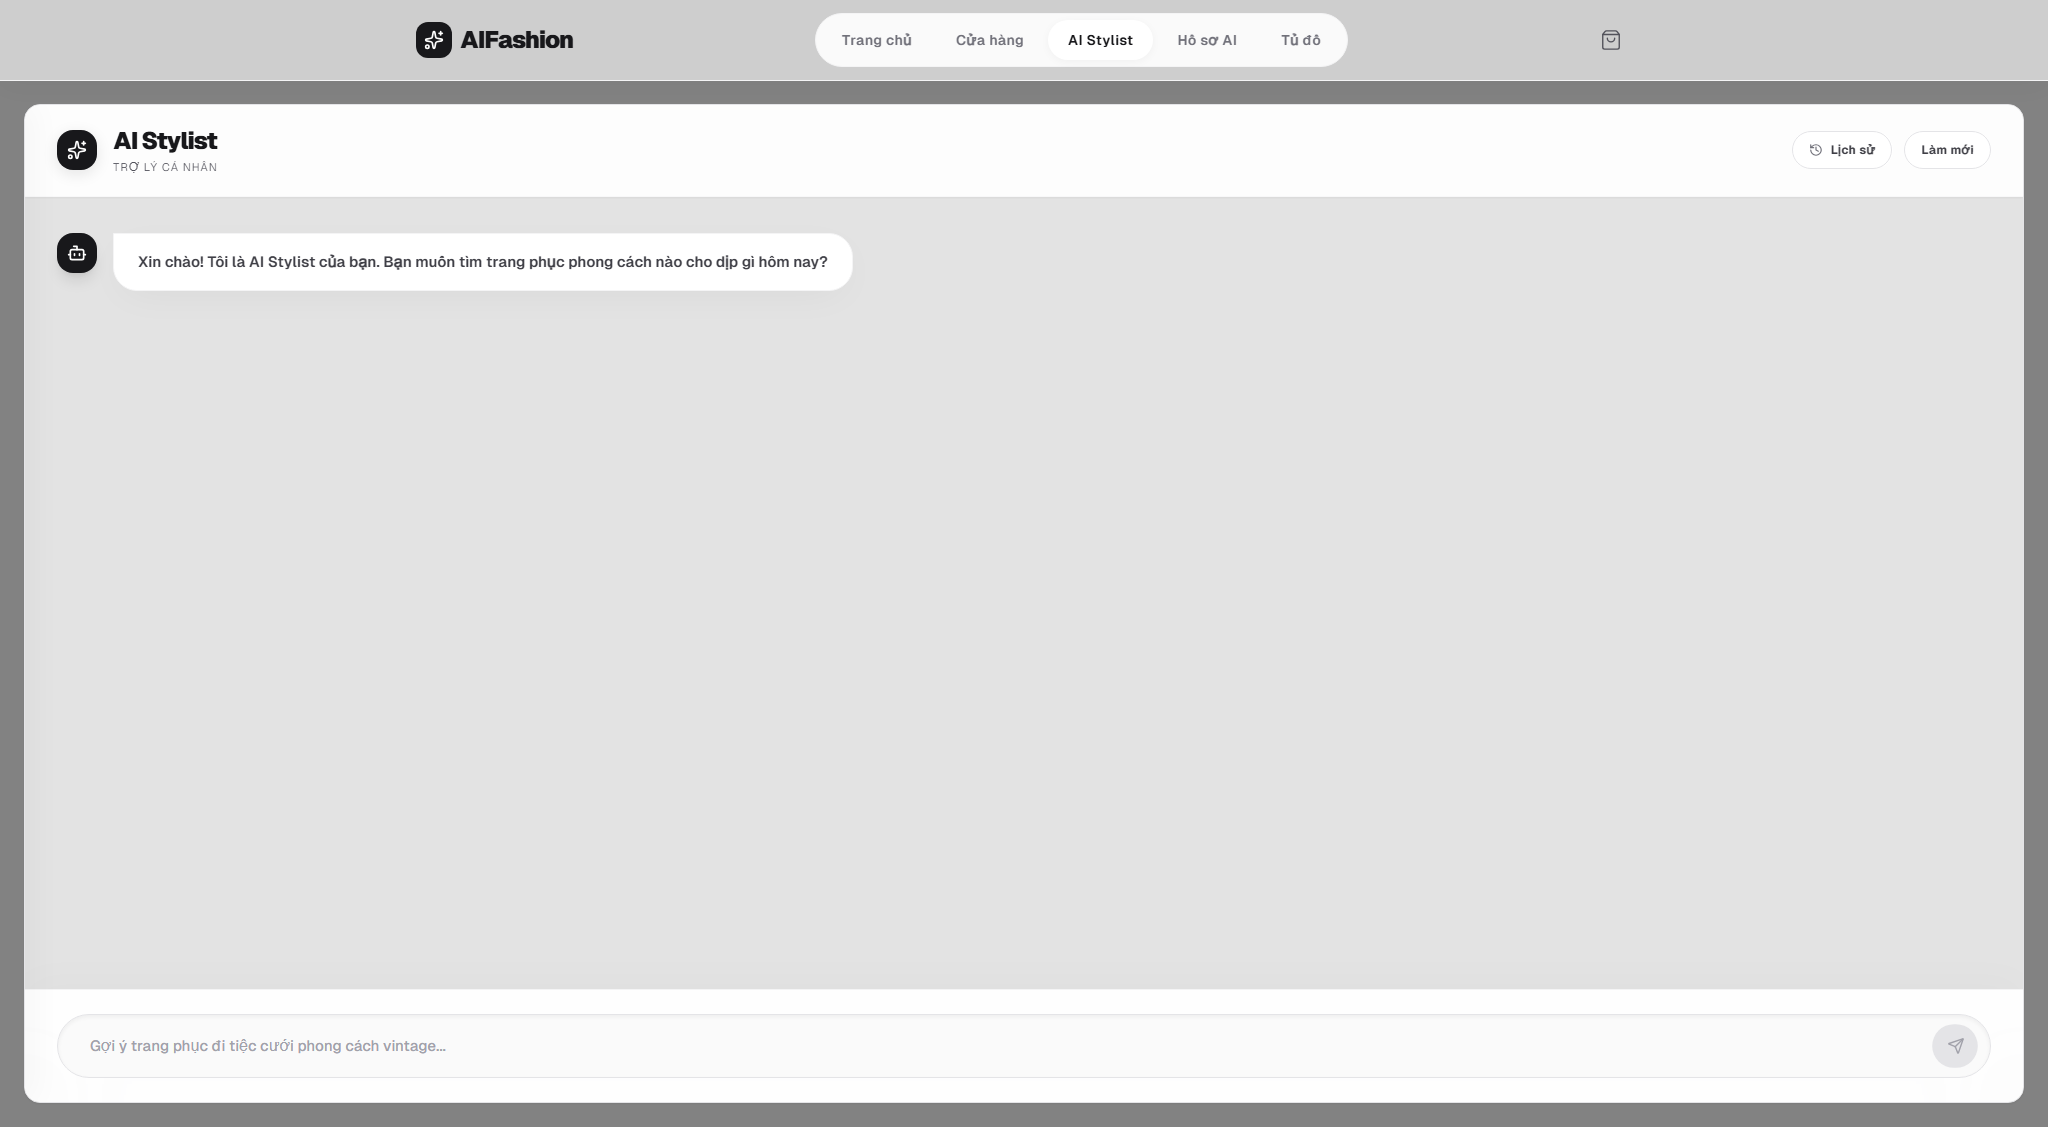
\includegraphics[width=0.95\textwidth]{Images/screenshots/ui_ai_stylist.png}
    \caption{Giao diện AI Stylist và khu vực hội thoại}
    \label{fig:ui-ai-stylist}
\end{figure}

\begin{figure}[H]
    \centering
    \begin{minipage}[t]{0.49\textwidth}
        \centering
        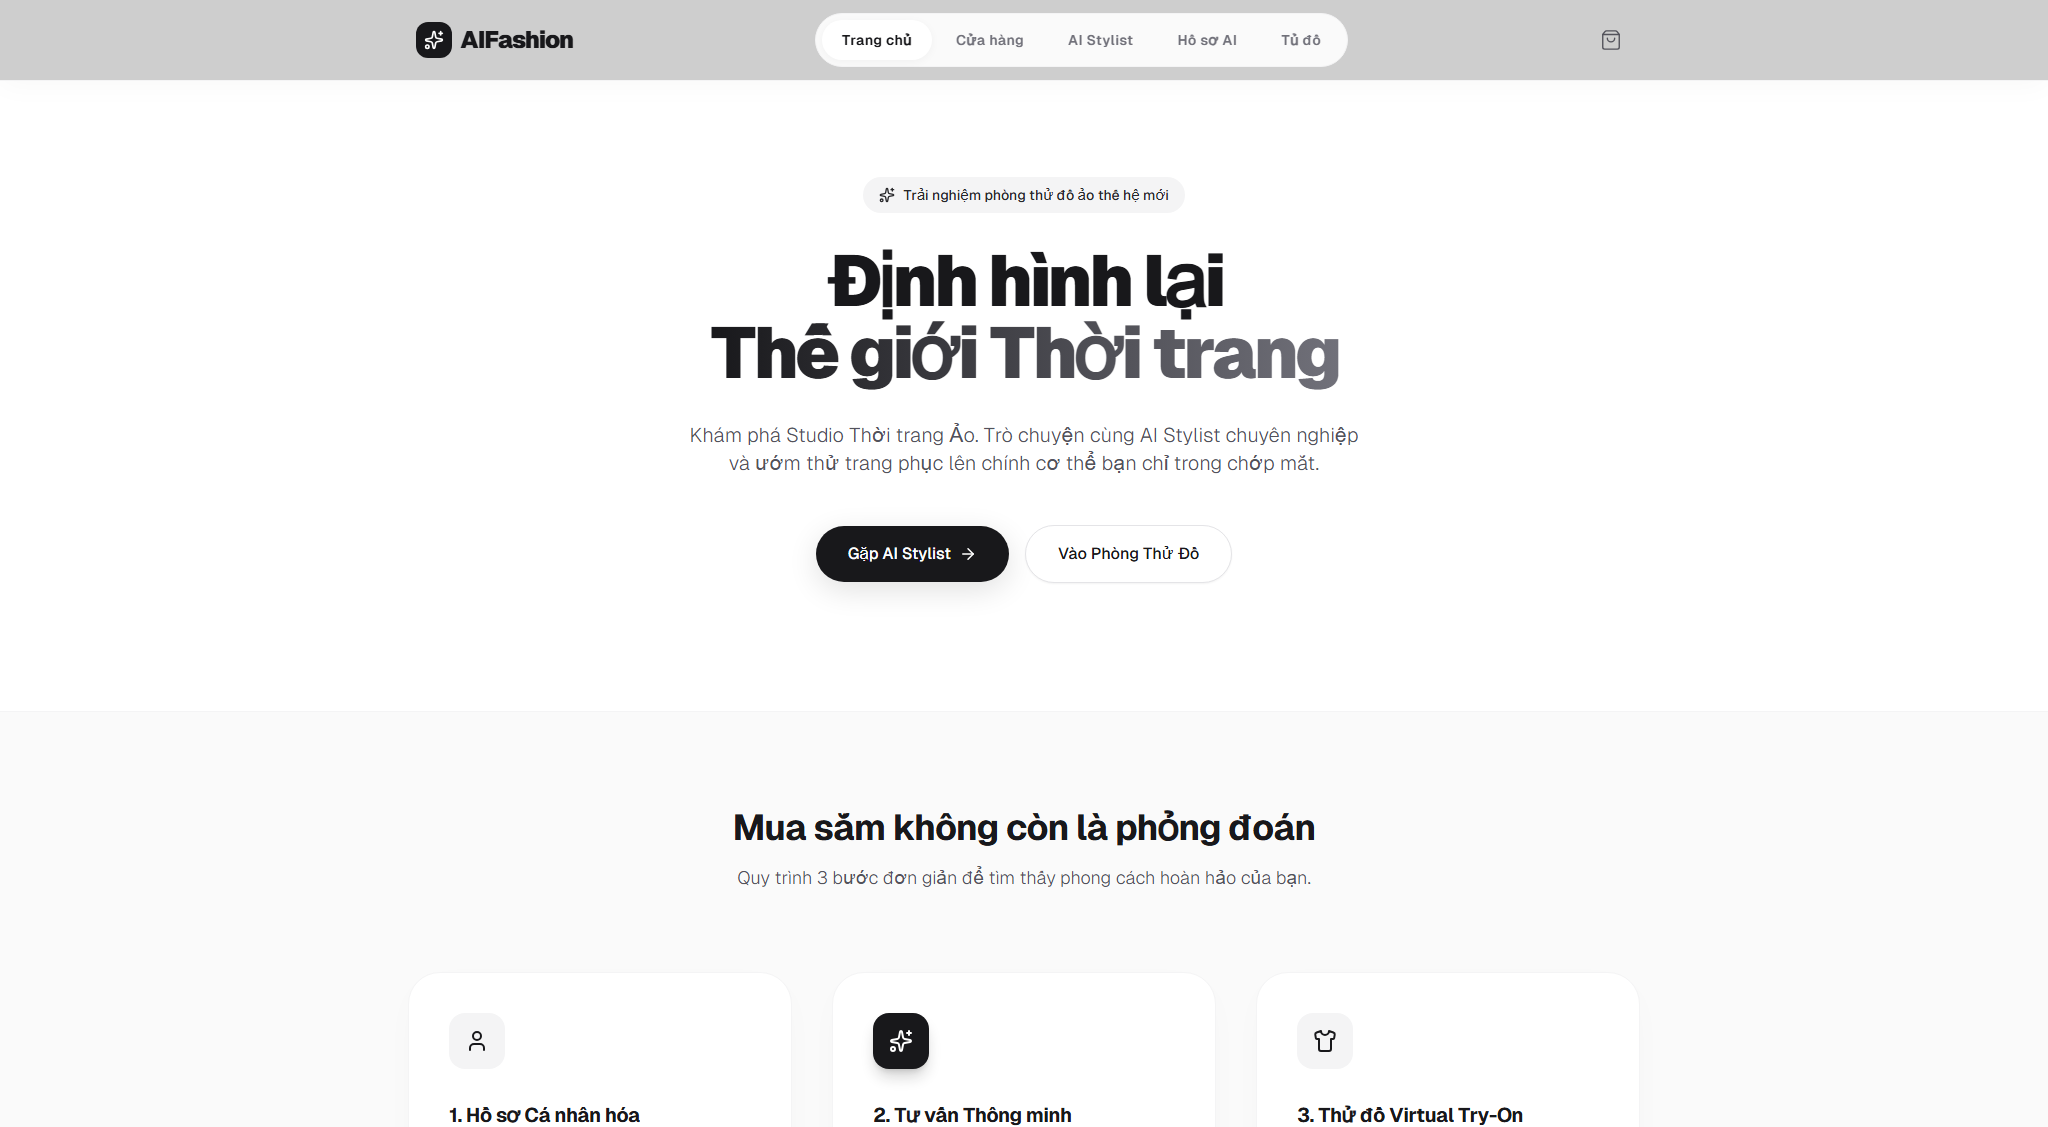
\includegraphics[width=\linewidth]{Images/screenshots/ui_home.png}
        \par\smallskip
        \small (a) Trang chủ
    \end{minipage}
    \hfill
    \begin{minipage}[t]{0.49\textwidth}
        \centering
        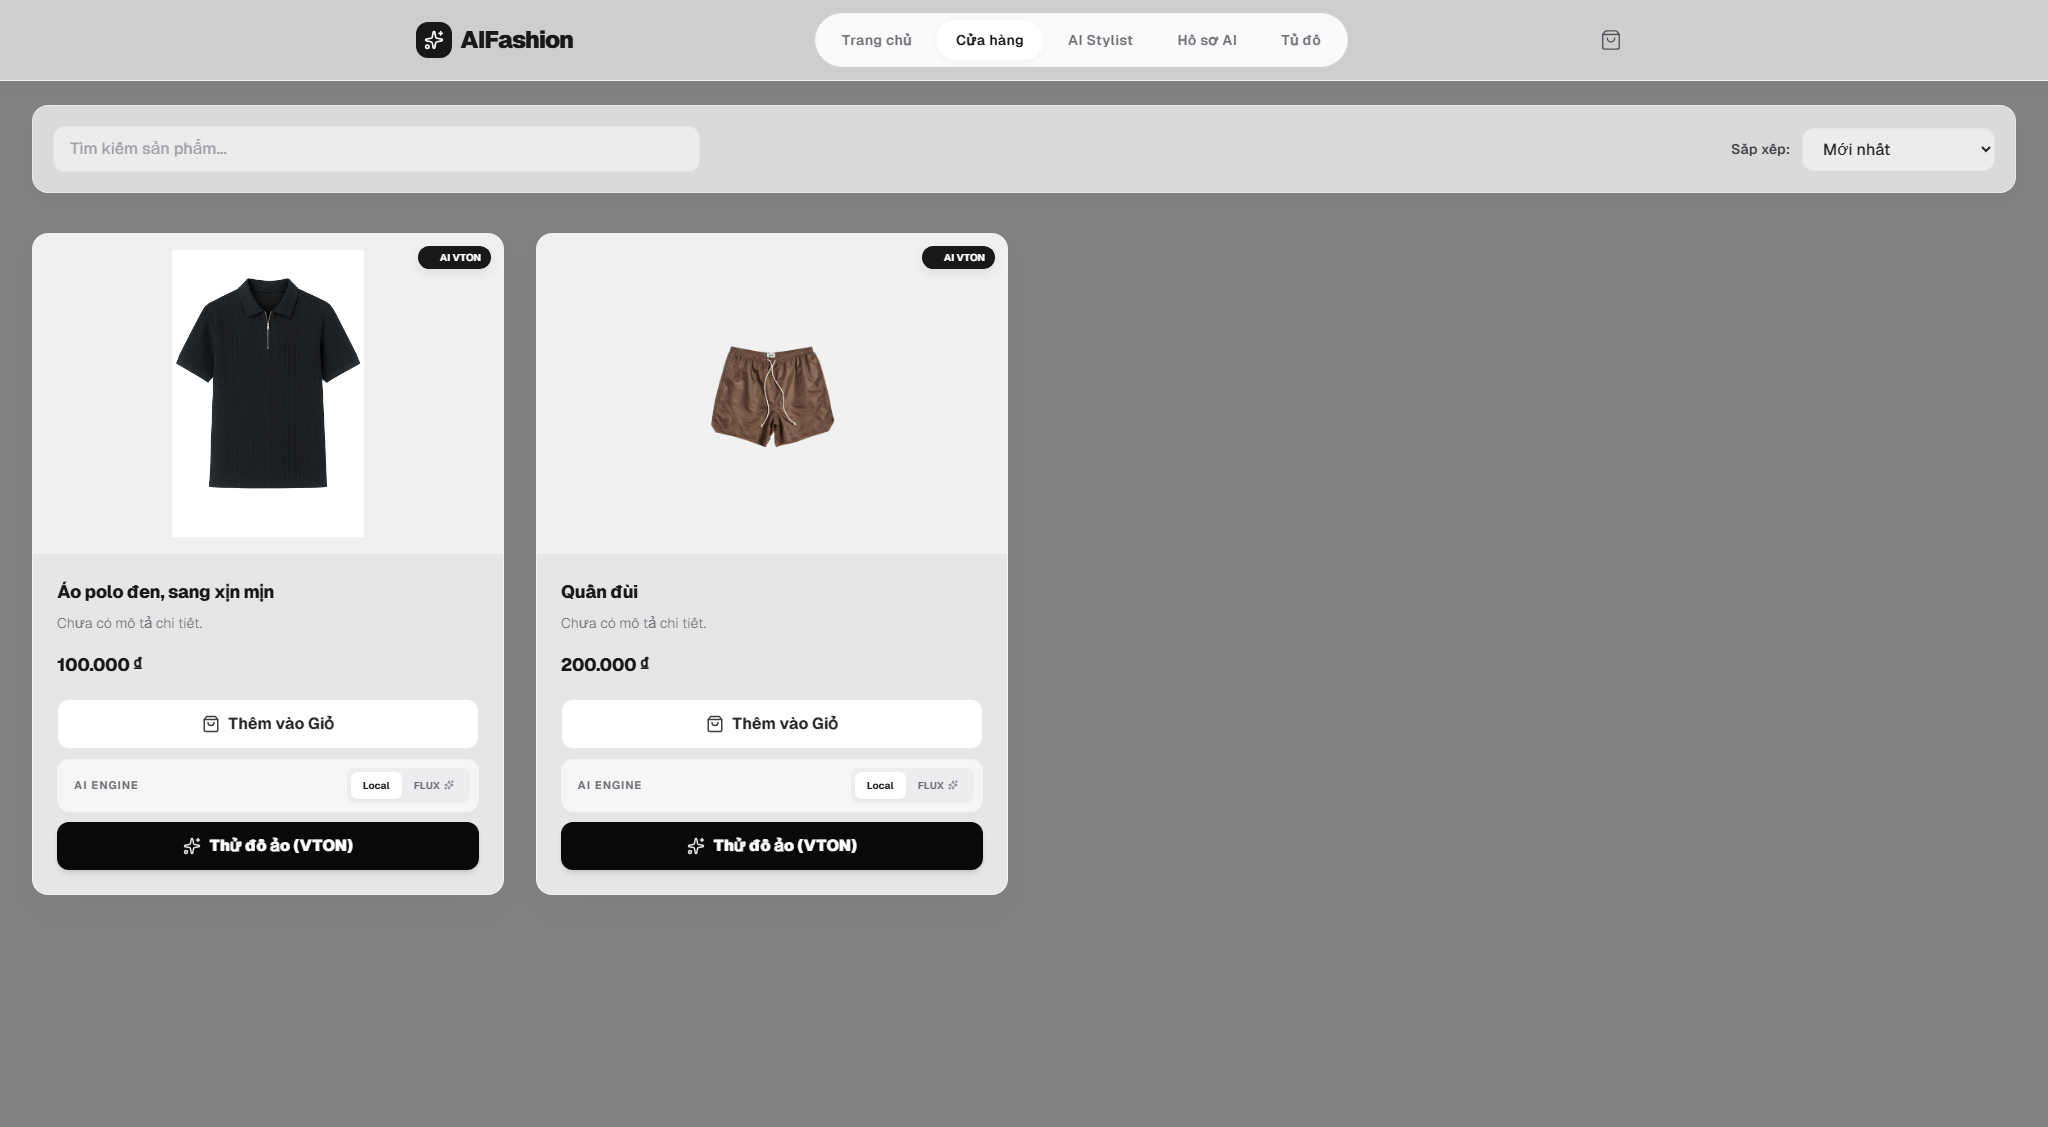
\includegraphics[width=\linewidth]{Images/screenshots/ui_products.png}
        \par\smallskip
        \small (b) Trang cửa hàng
    \end{minipage}
    \caption{Các màn hình cửa hàng chính}
    \label{fig:ui-storefront}
\end{figure}

\begin{figure}[H]
    \centering
    \begin{minipage}[t]{0.49\textwidth}
        \centering
        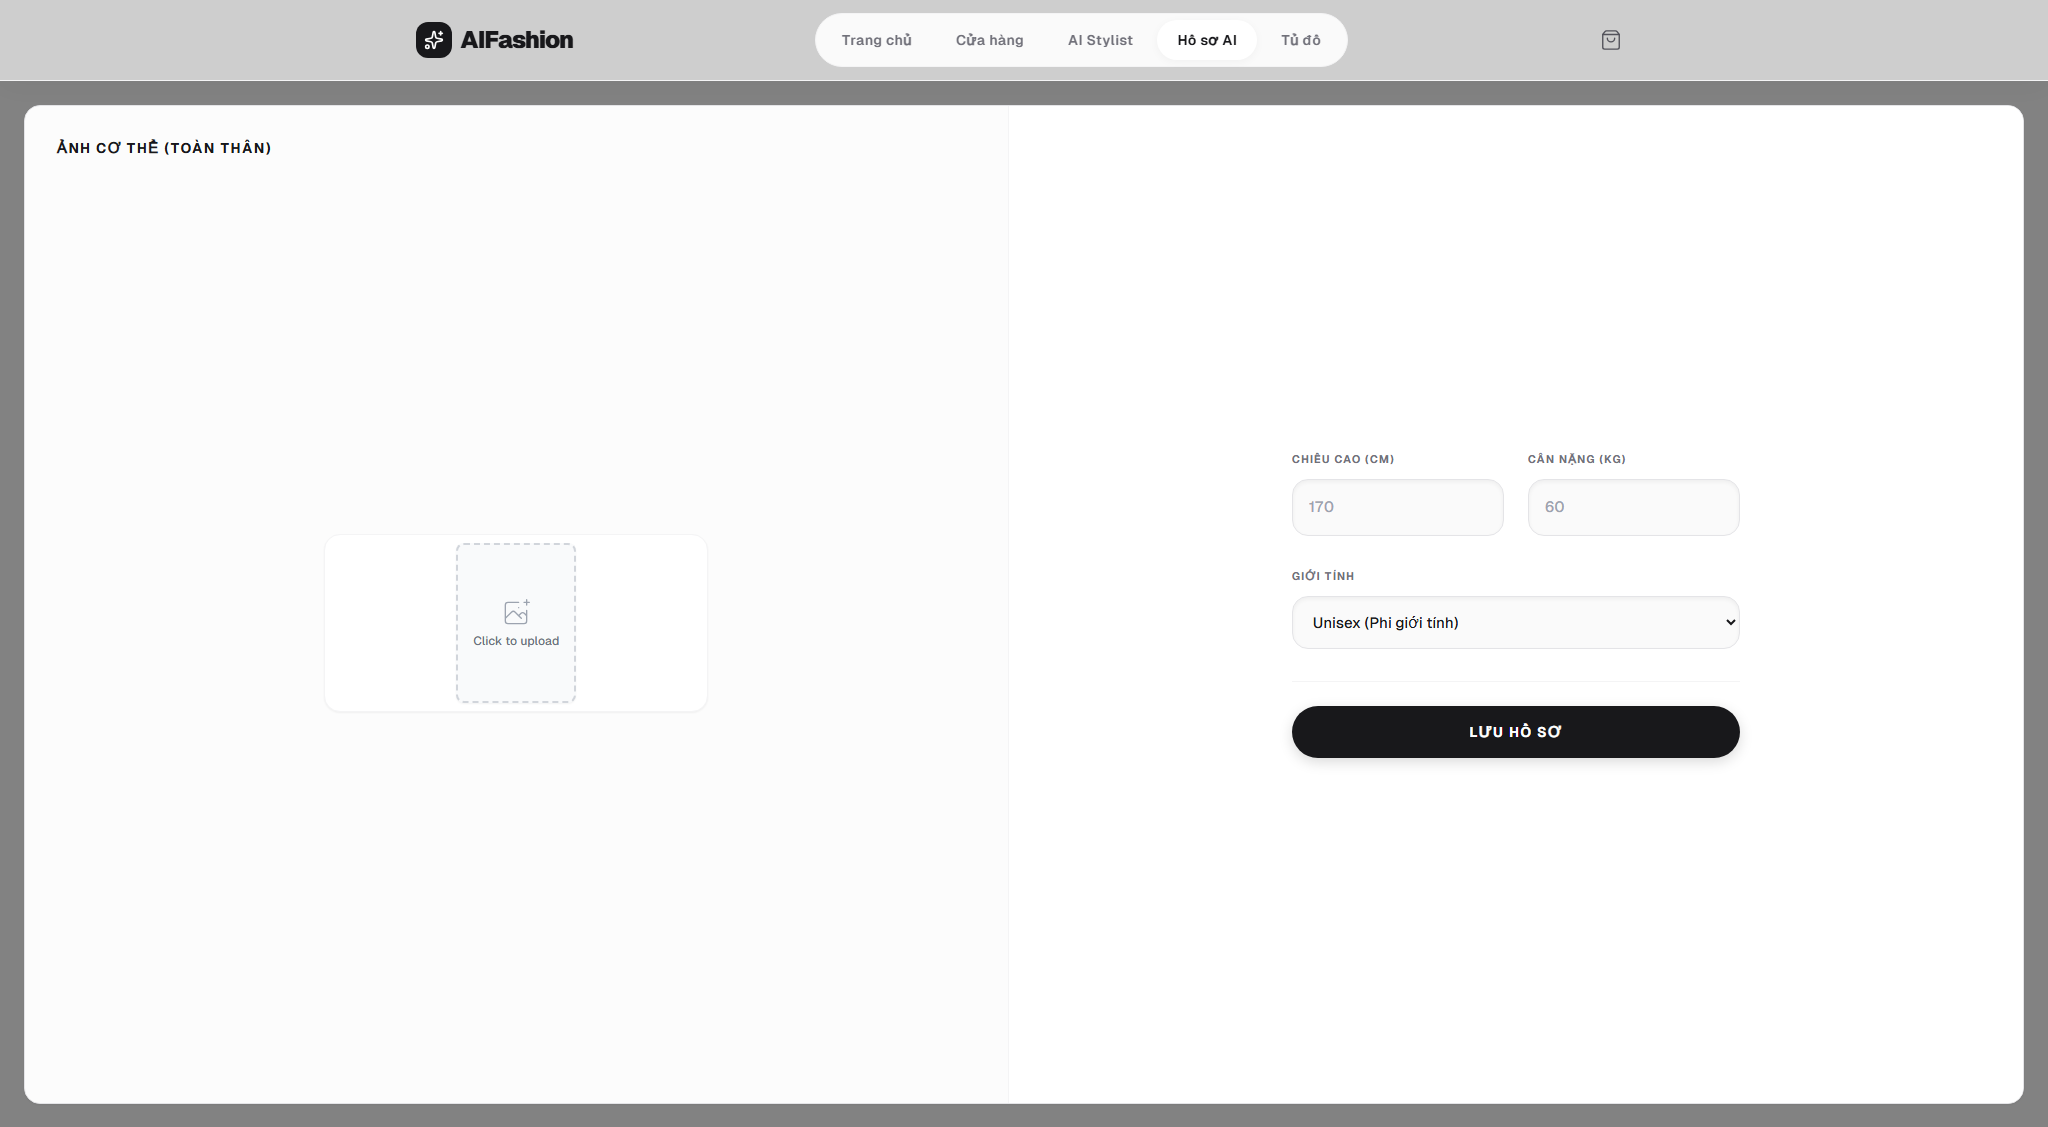
\includegraphics[width=\linewidth]{Images/screenshots/ui_ai_profile.png}
        \par\smallskip
        \small (a) Hồ sơ AI
    \end{minipage}
    \hfill
    \begin{minipage}[t]{0.49\textwidth}
        \centering
        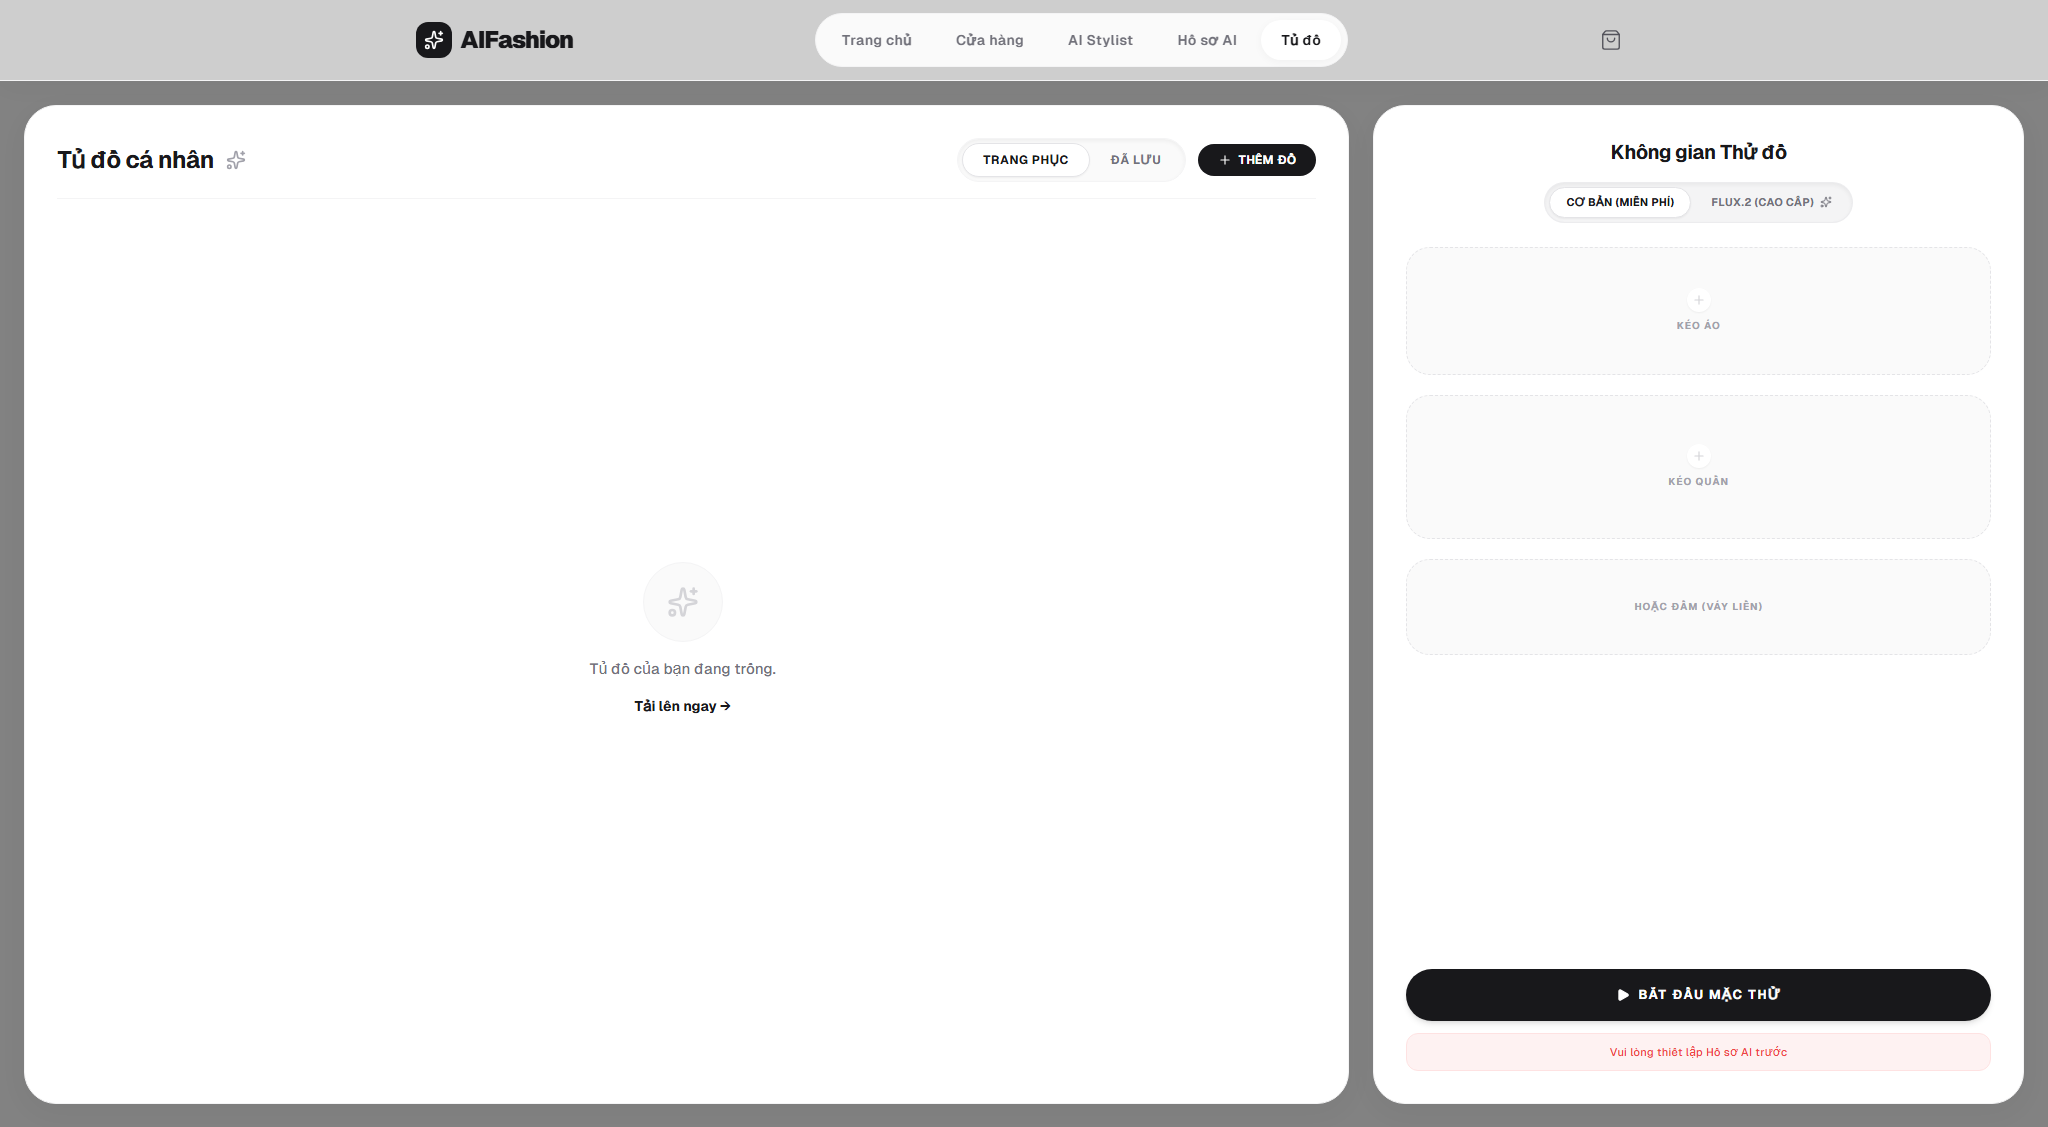
\includegraphics[width=\linewidth]{Images/screenshots/ui_wardrobe.png}
        \par\smallskip
        \small (b) Tủ đồ và không gian thử đồ
    \end{minipage}
    \caption{Giao diện hồ sơ AI và tủ đồ cá nhân}
    \label{fig:ui-profile-wardrobe}
\end{figure}

\medskip

Giao diện chỉ đảm nhiệm trình bày và thu thập thao tác. Các quyết định nghiệp vụ như kiểm tra sản phẩm, tạo tác vụ VTON hoặc lưu phiên tư vấn được đặt tại MedusaJS.

\section{Cài đặt hệ thống nghiệp vụ MedusaJS}

MedusaJS 2.14 và TypeScript được sử dụng để quản lý dữ liệu thương mại điện tử, cung cấp API cho giao diện và điều phối các luồng AI \cite{medusa}. Mô-đun \code{aiPersonalization} tập trung các thực thể hồ sơ AI, tủ đồ, phiên tư vấn và tác vụ VTON trong một phạm vi nghiệp vụ riêng.

\medskip

Các tuyến API tùy chỉnh dưới \code{apps/api-medusa/src/api/v1} được chia theo chức năng. Nhóm hồ sơ và tủ đồ tiếp nhận ảnh, chuẩn hóa định dạng, lưu bản ghi và phát sự kiện đồng bộ vector. Nhóm AI Stylist gọi dịch vụ AI, kiểm tra sản phẩm được đề xuất, bổ sung dữ liệu giao dịch và lưu phiên tư vấn. Nhóm VTON tạo tác vụ, phát thông điệp RabbitMQ và cập nhật trạng thái khi nhận kết quả.

\medskip

Cách tổ chức này đặt quyền kiểm soát nghiệp vụ tại Medusa. Dịch vụ AI chỉ trả kết quả phân tích hoặc sinh ảnh; dữ liệu sản phẩm, phiên người dùng và trạng thái tác vụ vẫn được Medusa kiểm tra trước khi cung cấp cho giao diện.

\section{Cài đặt dịch vụ AI FastAPI}

Dịch vụ AI được xây dựng bằng FastAPI và đặt trong \code{apps/ai-service} \cite{fastapi}. Khi khởi động, dịch vụ kết nối LanceDB, đăng ký các tuyến API nội bộ và khởi tạo bộ tiêu thụ RabbitMQ. Những phụ thuộc VTON có kích thước lớn được nạp trong luồng nền để các thành phần cơ bản có thể sẵn sàng trước.

\medskip

Ba nhóm thông điệp chính được xử lý độc lập: đồng bộ sản phẩm, đồng bộ tủ đồ và tác vụ VTON. Các lược đồ Pydantic kiểm soát dữ liệu đầu vào và đầu ra của API nội bộ, giúp phát hiện sớm trường thiếu hoặc sai kiểu trước khi dữ liệu được chuyển giữa Medusa, mô hình AI và LanceDB.

\section{Tích hợp các luồng chức năng chính}

Sau khi ba thành phần chính được cài đặt, hệ thống tích hợp chúng thành các luồng chức năng xuyên suốt giữa giao diện, Medusa, RabbitMQ, LanceDB và dịch vụ AI.

\medskip

\subsection{Đồng bộ dữ liệu sang LanceDB}

Khi sản phẩm được tạo hoặc cập nhật, \code{product-sync.ts} phát thông điệp vào \code{product_metadata_sync} qua RabbitMQ \cite{rabbitmq}. Dịch vụ AI sử dụng Gemini để trích xuất thuộc tính thời trang, tạo vector nhúng bằng CLIP và ghi dữ liệu vào \code{products_vector}. Bản ghi cũ của cùng \code{product_id} được thay thế trước khi ghi mới để tránh trùng lặp.

\medskip

Tủ đồ cá nhân được đồng bộ theo quy trình tương tự. Ảnh do người dùng tải lên được phân tích để suy luận danh mục, màu sắc, họa tiết và chất liệu; kết quả cùng vector nhúng được lưu trong \code{closet_vector}. Mỗi bản ghi luôn gắn với định danh chủ sở hữu để giới hạn phạm vi truy hồi.

\subsection{AI Stylist}

AI Stylist sử dụng \code{GeminiAnalyzerAdapter} để phân tích truy vấn, sinh phương án phối đồ và trích xuất thuộc tính thời trang. Sau bước phân tích ý định, \code{VectorSearch.global_search} truy hồi ứng viên từ sản phẩm cửa hàng và tủ đồ cá nhân. Tập ứng viên được truyền cho Gemini để sinh phương án phối đồ có cấu trúc.

\medskip

Chỉ dẫn cho mô hình được tách thành hai nhiệm vụ: phân tích yêu cầu và lựa chọn trang phục. Mô hình chỉ được chọn sản phẩm thuộc tập ứng viên, ưu tiên tủ đồ cá nhân và giới hạn số lớp có thể thử bằng VTON. Medusa tiếp tục kiểm tra định danh và bổ sung dữ liệu giao dịch, nhờ đó phần giải thích luôn gắn với sản phẩm thực tế.

\subsection{Virtual Try-On và cập nhật kết quả bằng SSE}

VTON hỗ trợ hai bộ xử lý. \code{LocalCatVTONAdapter} tải CatVTON, tạo mặt nạ khi cần và chạy suy luận trên máy cục bộ \cite{catvton}. \code{CloudFluxVTONAdapter} chuyển ảnh thành dữ liệu phù hợp, gọi FLUX.2 qua Replicate và tải ảnh kết quả về dịch vụ AI \cite{replicate}. Cả hai bộ xử lý tuân theo cùng hợp đồng giao tiếp nên phần điều phối không phụ thuộc trực tiếp vào mô hình cụ thể.

\medskip

Ảnh kết quả được lưu trong thư mục dữ liệu của dịch vụ AI và cung cấp qua địa chỉ tệp tĩnh, chẳng hạn \code{/static/vton/result_<job_id>.png}. Đây là giải pháp phù hợp với phạm vi bản triển khai tối thiểu; môi trường vận hành thực tế cần chuyển sang kho đối tượng dùng chung.

\medskip

Giao diện mở \code{EventSource} tới \code{/v1/stream/vision-results} trước khi tạo tác vụ. Khi Medusa nhận thông điệp từ \code{ai_vision_results}, \code{VisionOrchestrator} cập nhật trạng thái và \code{VisionSSEManager} gửi sự kiện \code{vision_update} tới người dùng tương ứng \cite{sse-mdn}. Thứ tự này giảm khả năng bỏ lỡ sự kiện và cho phép giao diện phản ánh liên tục trạng thái chờ, đang xử lý, hoàn tất hoặc thất bại.

\subsection{Thanh toán mô phỏng bằng Saga}

Luồng thanh toán phía Medusa được cài đặt bằng Medusa Workflow SDK. Quy trình gồm giữ tồn kho, tạo đơn hàng chờ xử lý, xử lý thanh toán mô phỏng và hoàn tất đơn hàng. Khi bước thanh toán thất bại, các hàm bù được thực thi để kiểm tra khả năng hoàn tác của quy trình Saga.

\medskip

Phần cài đặt này mới hoàn thành ở phía hệ thống nghiệp vụ; tuyến gọi từ giao diện chưa được thống nhất hoàn toàn với API Medusa. Vì vậy, thanh toán hiện đóng vai trò minh họa quy trình nghiệp vụ và chưa được xem là quy trình đầu cuối hoàn chỉnh.

\clearpage
